\documentclass[12pt, handout]{beamer}

\usetheme{Boulder}


\title{Unit testing with IDL}
\subtitle{Using mgunit to unit test code in IDL}
\author{Michael D. Galloy}
\institute[Tech-X Corporation]{Tech-X Corporation\\ Boulder, CO}
\titlegraphic{
\includegraphics[width=1.5cm]{TechX_logo.png}\hspace*{7.5cm}~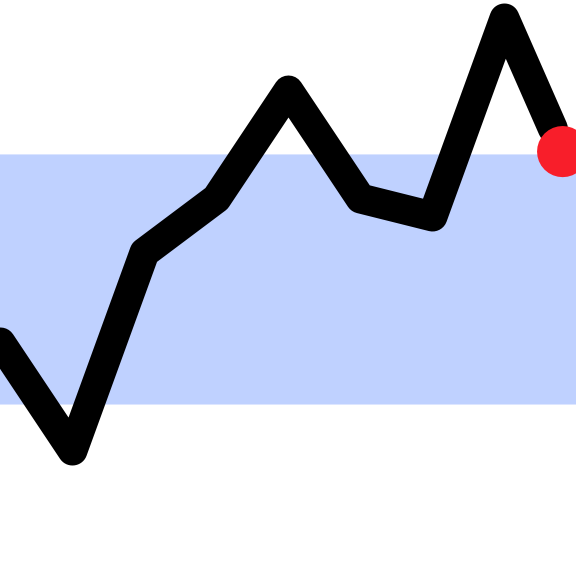
\includegraphics[width=1.5cm]{favicon-nogrid.png}}
%\logo{
\includegraphics[width=1cm]{TechX_logo.png}}

\date{11 November 2013}


\begin{document}


\begin{frame}[plain]
  \titlepage
\end{frame}


\section{Introduction}
\subsection*{}

\begin{frame}
  \tableofcontents
\end{frame}

\begin{frame}{Why test?}
Advantages:
  \begin{enumerate}
    \item find problems early
    \item provide safety for making changes
    \item provide an example of using the code
    \item design interface (Test-Driven Development)
    \item find problems later (version control helps)
  \end{enumerate}
You have to run the code at some point to see if it works. Why not put that in a file as a unit test that can be run at any time?
\end{frame}

\begin{frame}{Legacy code}
  \begin{quote}All code is legacy code.\end{quote}
When to write a unit test? Every time you ``touch'' a routine:
  \begin{enumerate}
    \item creating or modifying a routine/class
    \item after finding a bug
    \item after looking at it
    \item after calling it
  \end{enumerate}
\end{frame}

\begin{frame}[t, fragile]
  \frametitle{mgunit project}
  \begin{itemize}
    \item Available on GitHub:

\begin{lstlisting}
  github.com/mgalloy/mgunit
\end{lstlisting}

    \item At least 6 years old, moved to GitHub about a year ago
    \item Goal: quick and easy
    \begin{enumerate}
      \item use name conventions over explicit specifications
      \item reasonable defaults
    \end{enumerate}
  \end{itemize}
\end{frame}


\section{Using mgunit}
\subsection{Basics}

\begin{frame}[t, fragile]
  \frametitle{Tests and test cases}
  \begin{enumerate}
    \item Create a class for each test case that inherits from {\em MGutTestCase} (put it in your {\tt !path})
    \item Tests are methods which are:
      \begin{itemize} 
        \item functions
        \item method name starts with ``test''
      \end{itemize}
    \item Test results:
      \begin{itemize}
        \item pass if returns 1
        \item fail if returns 0 or crashes ({\tt ASSERT} fails)
        \item skips if {\tt ASSERT} fails with {\em SKIP} set
      \end{itemize}
  \end{enumerate}
\end{frame}

\begin{frame}[t, fragile]
  \frametitle{Simple test case}

\begin{lstlisting}[basicstyle=\ttfamily\fontsize{10pt}{10pt}\selectfont]
function gpurepmat_ut::test_1d
  ; do testing
  return, 1
end

function gpurepmat_ut::test_2d
  ; do testing
  return, 1
end

pro gpurepmat_ut__define
  define = { gpurepmat_ut, inherits GPUutTestCase }
end
\end{lstlisting}

\end{frame}


\begin{frame}[t, fragile]
  \frametitle{Running tests}

Run a single test case:
\begin{lstlisting}
  IDL> mgunit, 'gpurepmat_ut'
\end{lstlisting}
Run a single test:
\begin{lstlisting}
  IDL> mgunit, 'gpurepmat_ut.test_2d'
\end{lstlisting}
Run a list of test cases:
\begin{lstlisting}
  IDL> mgunit, ['gpurepmat_ut', 'gputotal_ut']
\end{lstlisting}

\end{frame}

\begin{frame}{Output}
For example, from the IDL prompt:
\begin{center}
  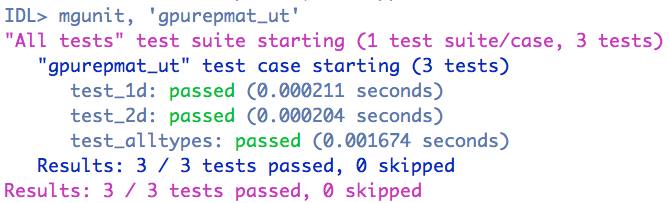
\includegraphics[scale=0.45]{cli-output.png}
\end{center}
\end{frame}

\begin{frame}[t, fragile]
  \frametitle{{\tt ASSERT} routine}

The {\tt ASSERT} routine immediately causes a test to fail (or optionally skip the test) if the {\em condition} is not true:
\begin{lstlisting}
  ASSERT, condition $
          [, msg] [, arg1] [, arg2] [, arg3] $
          [, /SKIP]
\end{lstlisting}
For example:
\begin{lstlisting}
  assert, result eq standard, $
          'incorrect result: %d', result
\end{lstlisting}

\end{frame}

\subsection{More features}

\begin{frame}[t, fragile]
  \frametitle{More features}
  \begin{description}
    \item[Test suites] collection of tests that can be run with a single name
    \item[Fixtures] {\em setup}/{\em teardown} methods run before and after every test
    \item[Test runners] different output formats: text files, HTML, XML, GUI
  \end{description}
\end{frame}


\section{Examples}
\subsection*{}

\begin{frame}[t, fragile]
  \hypertarget{examples}{}
  \frametitle{Examples}
  Examples will come from:

  \begin{description}
    \item[GPULib] CUDA bindings for IDL
\begin{lstlisting}
  txcorp.com/home/gpulib
\end{lstlisting}
\hyperlink{gpulib}{\beamergotobutton{go to GPULib}}

    \item[mglib] My personal library for analysis, file I/O, visualization, collections, utility routines, string manipulation, \ldots
\begin{lstlisting}
  gitgub.com/mgalloy/mglib
\end{lstlisting}
  \end{description}
\end{frame}

\begin{frame}[t, fragile]
  \frametitle{gpurepmat\_ut::test\_1d}

\begin{lstlisting}[basicstyle=\ttfamily\fontsize{8pt}{8pt}\selectfont]
function gpurepmat_ut::test_1d
  compile_opt strictarr

  dx = gpufindgen(5, ERROR=err)
  assert, err eq 0, 'CUDA error: %s', gpu_errormessage(err)

  dresult = gpurepmat(dx, 3, ERROR=err)
  assert, err eq 0, 'CUDA error: %s', gpu_errormessage(err)

  result = gpugetarr(dresult, ERROR=err)
  assert, err eq 0, 'CUDA error: %s', gpu_errormessage(err)

  gpufree, [dx, dresult]
\end{lstlisting}
\end{frame}

\begin{frame}[t, fragile]
  \frametitle{gpurepmat\_ut::test\_1d}

\begin{lstlisting}[basicstyle=\ttfamily\fontsize{8pt}{8pt}\selectfont]
  type = size(result, /type)
  ndims = size(result, /n_dimensions)
  dims = size(result, /dimensions)

  standard = [[0., 1., 2., 3., 4.], $
              [0., 1., 2., 3., 4.], $
              [0., 1., 2., 3., 4.]]

  assert, type eq 4L, 'incorrect type: %d', type
  assert, ndims eq 1, 'incorrect number of dimensions: %d', ndims
  assert, array_equal(dims, [15]), 'incorrect dimensions: [%s]', $
          strjoin(strtrim(dims, 2), ',')
  assert, array_equal(result, standard), 'incorrect value'

  return, 1
end
\end{lstlisting}
\end{frame}


\subsection{Skipping tests}

\begin{frame}[t, fragile]
  \frametitle{Skipping tests (GPULib)}
For example, don't test double precision on a graphics card that is not capable of it:
\begin{lstlisting}
  assert, !gpu.mode eq 0 || gpuDoubleCapable(), $
          'CUDA device not double capable', $
          /skip
\end{lstlisting}
We can run the GPULib test suite on laptops and servers with greatly varying capabilities.
\end{frame}

\begin{frame}[t, fragile]
  \frametitle{Skipping tests (mglib)}
Don't test a routine that requires a higher version of IDL than is present:
\begin{lstlisting}
  assert, mg_idlversion(require='8.0'), /skip, $
          'test requires IDL 8.0, %s present', $
          !version.release
\end{lstlisting}
Don't test a routine in a DLM if the DLM is not available:
\begin{lstlisting}
  assert, self->have_dlm('mg_analysis'), $
          'MG_ANALYSIS DLM not found', $
          /skip
\end{lstlisting}

\end{frame}

\subsection{Test suites}

\begin{frame}[t, fragile]
  \hypertarget{suites}{}
  \frametitle{Test suites (collections of test cases)}
  \begin{enumerate}
    \item Create a class, say {\em mglib\_uts}, that inherits from {\em MGutTestSuite}
    \item To automatically collect all {\em \_ut\_\_define.pro} files in its directory and subdirectories, just all
\begin{lstlisting}
  self->add, /all
\end{lstlisting}
to the {\em init} method
    \item Run with
\begin{lstlisting}
  IDL> mgunit, 'mglib_uts'
\end{lstlisting}
  \end{enumerate}
\end{frame}

\begin{frame}[fragile]
  \frametitle{mglib\_uts\_\_define.pro}
\begin{lstlisting}[basicstyle=\ttfamily\fontsize{10pt}{10pt}\selectfont]
function mglib_uts::init, _extra=e
  compile_opt strictarr

  if (~self->mguttestsuite::init(_strict_extra=e)) then $
    return, 0
  self->add, /all

  return, 1
end

pro mglib_uts__define
  compile_opt strictarr

  define = { mglib_uts, inherits MGutTestSuite }
end
\end{lstlisting}
\end{frame}

\subsection{Fixtures}

\begin{frame}
  \frametitle{Inherit from a subclass of {\em MGutTestCase}}
Unit tests in mglib inherit from {\em MGutLibTestCase}; unit tests in GPULib inherit from {\em GPUutTestCase}.

This allows you to:
\begin{enumerate}
  \item set {\em setup}/{\em teardown} methods for all test cases at once (particularly for checking for memory leaks)
  \item set member variables for the location of resource files, common error tolerances, etc.
  \item define helper methods that are used throughout the tests (I have a {\em have\_dlm} method in {\em MGutTestCase})
\end{enumerate}
\end{frame}

\begin{frame}[t, fragile]
  \frametitle{Setup}

For example, the mglib tests check heap memory before\ldots
\begin{lstlisting}[basicstyle=\ttfamily\fontsize{10pt}{10pt}\selectfont]
pro mgutlibtestcase::setup
  compile_opt strictarr

  mg_heapinfo, n_pointers=nptrs, n_objects=nobjs
  self.nptrs = nptrs
  self.nobjs = nobjs
end
\end{lstlisting}
\end{frame}

\begin{frame}[t, fragile]
  \frametitle{Teardown}

\ldots and compare to after the test is executed
\begin{lstlisting}[basicstyle=\ttfamily\fontsize{10pt}{10pt}\selectfont]
pro mgutlibtestcase::teardown
  compile_opt strictarr

  mg_heapinfo, n_pointers=nptrs, n_objects=nobjs
  assert, nptrs eq self.nptrs && nobjs eq self.nobjs, $
          'leaked %d pointers, %d objects', $
          nptrs - self.nptrs, $
          nobjs - self.nobjs
end
\end{lstlisting}
The GPULib tests also check for leaked GPU memory.
\end{frame}

\section{Conclusion}

\subsection{Tips}
\begin{frame}[t]{Tips}
  \begin{enumerate}
    \item Run tests {\em regularly}
    \item Follow the name conventions
    \item Inherit from a subclass of {\em MGutTestCase}
    \item Use descriptive names for test methods
    \item Skipping tests allows tests to run in a wide range of environments
    \item Keep tests fairly quick
  \end{enumerate}
\end{frame}

\subsection{Future work}
\begin{frame}[t]{Future work}
  \begin{enumerate}
    \item mgunit is fairly mature and not many extra features are currently planned
    \item Testing may be integrated into docs in some way, but that will probably be a feature of IDLdoc and separate from mgunit
    \item Any suggestions? Let me know/file an issue on GitHub.
  \end{enumerate}
\end{frame}

\begin{frame}{Thanks!}
  \begin{center}

{\huge Questions?} \\

\bigskip

{mgalloy@txcorp.com} \\
{michaelgalloy.com} \\
{@mgalloy} \\
~\\
{\em Modern IDL: A Guide to IDL Programming} \\
{modernidl.idldev.com} \\


\end{center}
\end{frame}

% for extra slides
\appendix

\begin{frame}[t]{GPULib 1.6.2}
\hypertarget{gpulib}{}

GPULib provides CUDA bindings for IDL performing GPU accelerated routines for:
\begin{itemize}
  \item Vector and matrix operations
  \item {\tt HISTOGRAM} and {\tt WHERE} routines
  \item 1D, 2D, and 3D FFTs (including batched)
  \item LAPACK linear algebra routines (MAGMA)
  \item Loading and executing custom CUDA code
\end{itemize}
See {\tt txcorp.com/home/gpulib} for more information

\hyperlink{examples}{\beamergotobutton{go to Examples}}
\end{frame}

\begin{frame}[t]{FastDL}
\begin{description}
  \item[TaskDL 2.4.0] Task farming for IDL
  \item[mpiDL 2.4.0] MPI bindings for IDL
\end{description}
\vspace{-2.25em}
\begin{center}
  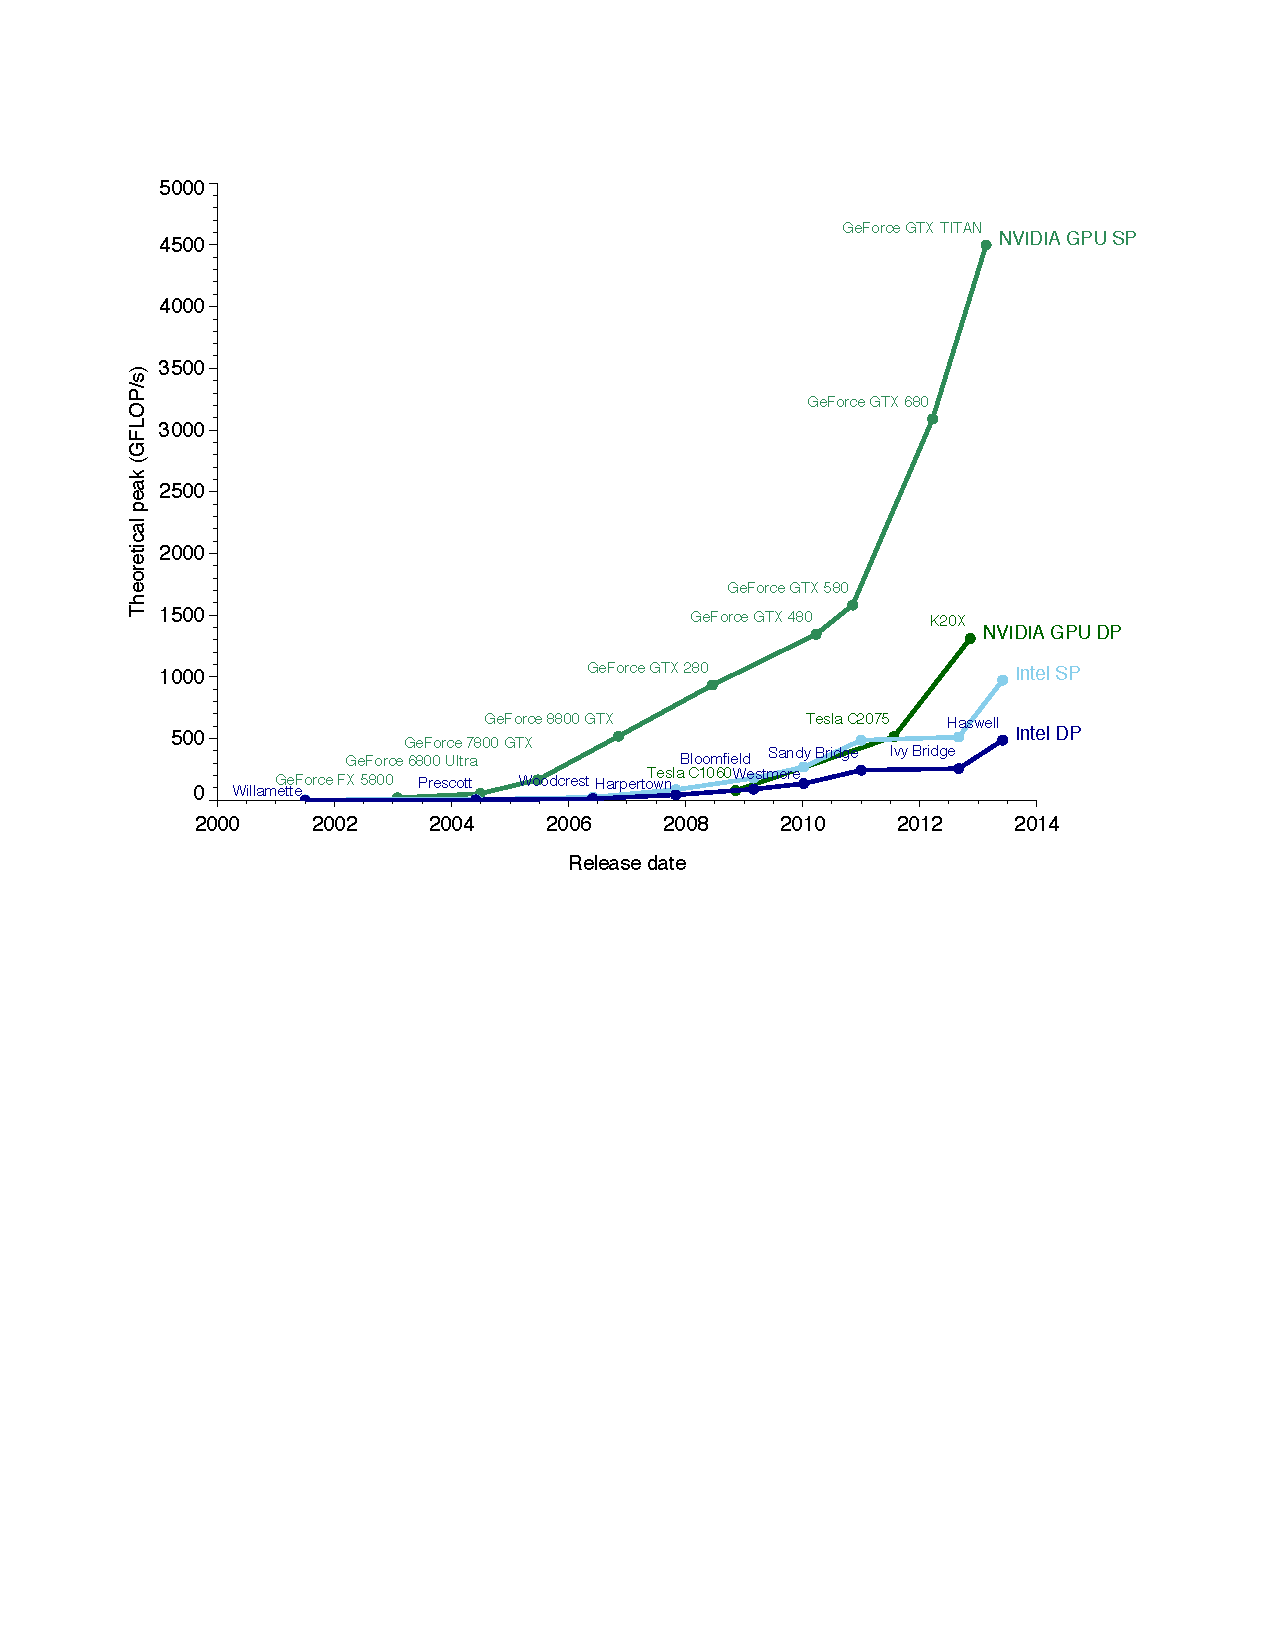
\includegraphics[scale=0.4]{cpu-vs-gpu.pdf}
\end{center}
\end{frame}

\begin{frame}[t, fragile]
  \frametitle{Open source IDL projects}

\begin{description}
  \item[IDLdoc 3.5.1] Documentation generation
\begin{lstlisting}
  github.com/mgalloy/idldoc
\end{lstlisting}
  \item[mgunit 1.3.0] Unit testing
\begin{lstlisting}
  github.com/mgalloy/mgunit
\end{lstlisting}
  \item[mglib] Personal library of miscellaneous routines
\begin{lstlisting}
  github.com/mgalloy/mglib
\end{lstlisting}
  \item[rIDL] More powerful command line
\begin{lstlisting}
  github.com/mgalloy/ridl
\end{lstlisting}
\end{description}
\end{frame}

\end{document}
